

\section{Bombardier}
\subsection{System architecture}
\frame
{
  \frametitle{Bombardier System architecture}
 \begin{center}
	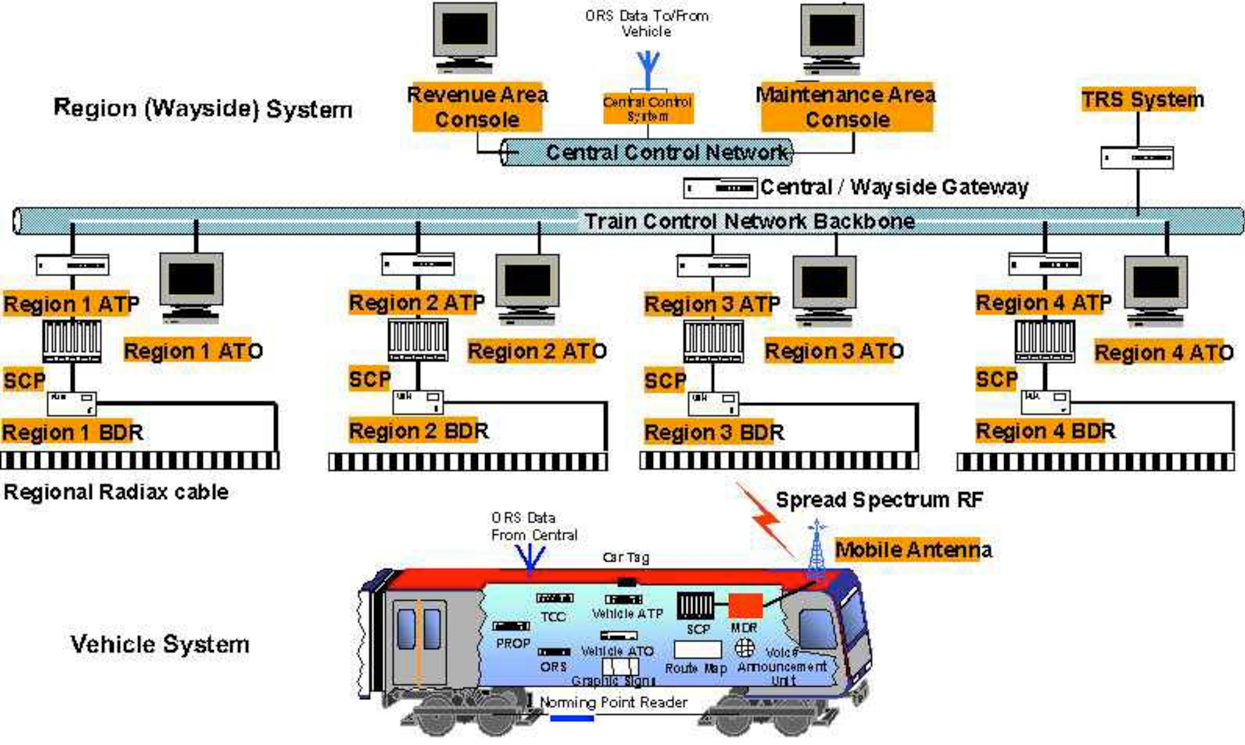
\includegraphics[scale=0.5]{./fig/BombadierArchitetture}
      \end{center}
   
}

\subsection{Operating mode, Safety and failure management}
\frame
{
\begin{block}<1->{Operating mode management}
CITYFLO 650 can also be used as an overlay train control system or resignalling % to upgrade existing fixed block (brown field) systems.
\end{block}
\begin{alertblock}<2->{Safety and failure management}
\begin{itemize}
\item \textbf{Full secondary signalling system using the conventional track circuits, interlockings and wayside signals}. 

The solution is based on the Bombardier EBI Lock 950 Computer Based Interlocking (CBI).
\item CITYFLO systems allow a \textbf{cold start-up}
\end{itemize}

 

   \end{alertblock}
}


\subsection{Communication and Interlocking}
\frame
{
  
\begin{block}<1->{Communication infrastructure and protocol}
\begin{itemize}
\item The RF communication uses either a leaky coaxial cable or Line of Sight (LOS) antenna network along the wayside that transmits data to the trains via their onboard mobile antennas.
\item The train has also an internal communication network, which uses the IEEE-1473 protocol.
\end{itemize}
\end{block}

\begin{block}<2->{Interlocking and wayside information integration}
\begin{itemize}
\item The CITYFLO 650 built-in interlocking function is \textbf{located with the regional wayside ATP}.


\item The CITYFLO 650 solution can either use the \textbf{built-in interlocking function or add optional EBI Lock computer-based interlocking for fall-back system capability} or adherence to local norms. 
\end{itemize}



   \end{block}
}

%System architecture
%Operating mode management
%Safety and failure management
%Communication infrastructure and protocol
%Interlocking and wayside information integration

\subsection{ATS functions}
\frame
{

  
\begin{block}<1->{ATS functions}
\begin{itemize}
\item Manual override requests {\footnotesize  (when the central operator substitutes the automatic system ATP or ATO)}
\item Management initiation and termination of service
\item Management of train schedules including dwell and headway control
\item Management of route assignments for normal operations and failure modes 
\item Train management (including skip station or station close) 
\item Remote set or reset of emergency brakes
\item Voice communication with the train and supervision
\item Control of any power distribution system (SCADA)
\end{itemize}
\end{block}
}


%ATS functions

\subsection{Headway, Train speed and train location determination }
\frame
{
  

\begin{block}<1->{Headway}
\begin{itemize}
\item {\scriptsize CITYFLO 650} is capable of less than 75 second headway
\item  \textmd{Metro Madrid Line} 1\&6: 101s/111s headway
 
\end{itemize}

   \end{block}
   
   \begin{block}<2->{Braking models and speed limit protection}
No Information

   \end{block}
   
      \begin{block}<3->{Train speed and train location determination}
      \begin{itemize}
       \item Tracks divided into entity called a ``{\scriptsize CITYFLO Segment}'' .  

For \textbf{example} suppose that a train was 25\% through segment \textbf{R}1\textbf{S}4 in �Moving Block Coordinate System� is \textbf{R}egion 1, \textbf{S}egment 4, and Offset 25.

\item A Norming Point is a {\small \textbf{Passive Tag containing Location Data}.
}\item A \textbf{Conflict Point} is defined as the end of movement authority.
\item Neihu-Muzha Line \textbf{maximum speed of 80 km/h}
\end{itemize}



   \end{block}
}

%Headway
%Braking models and speed limit protection
%Train speed and train location determination

\subsection{Door management, ATO functions and Service-oriented facilities}
\frame
{
  

\begin{block}<1->{Door management}
\begin{itemize}
\item Door control requests are issued by the ATO system (both onboard and wayside). 
\item  The ATO system allows precision stopping by the train at stations with a typical accuracy of +/- 15 cm 
\end{itemize}

   \end{block}
   
   \begin{block}<2->{ATO functions}
   \begin{itemize}
\item  Each Region has an independent ATO.
\item Ride Comfort Control, e.g. jerk limiting (VATO)
\item Stopping accuracy (VATO?
\item Speed profile (VATO)
\item Door Control Requests (RATO and VATO)
\item Onboard  and Wayside PIDs and PA (VATO and RATO)
\end{itemize}
   \end{block}
   
   }


%Door management
%ATO functions

\subsection{Service-oriented facilities}
\frame
{  
   
      \begin{block}<1->{Service-oriented facilities}
      \begin{itemize}
       \item Passenger information displays (PIDs)
  \item CCTV (Closed Circuit TV)
  \item Public announcement (PA)
  \item Radio
  \item Telecoms
\end{itemize}



   \end{block}
   
    \begin{block}<2->{}
   End
   \end{block}
}

%Service-oriented facilities
%qui
  %\begin{itemize}
  %\item<1-> Normal LaTeX class.
  %\item<2-> Easy overlays.
  %\item<3-> No external programs needed.      
  %\end{itemize}

